%
% Tutorial -- Getting Started with Digital Circuit Simulation
%
% Copyright (C) 2006 Mike Brinson <mbrin72043@yahoo.co.uk>
%
% Permission is granted to copy, distribute and/or modify this document
% under the terms of the GNU Free Documentation License, Version 1.1
% or any later version published by the Free Software Foundation.
%

% redefine subfigure caption
\renewcommand{\thesubfigure}{\thefigure(\alph{subfigure})}
\makeatletter
  \renewcommand{\@thesubfigure}{\thesubfigure:\space}
  \renewcommand{\p@subfigure}{}
\makeatother

% redefine subtable caption
\renewcommand{\thesubtable}{\thetable(\alph{subtable})}
\makeatletter
  \renewcommand{\@thesubtable}{\thesubtable:\space}
  \renewcommand{\p@subtable}{}
\makeatother

\tutsection{Introduction}

On 21 January 2006 Qucs 0.0.8 was released by the Qucs development
team.  This is the first version of the package to include digital
circuit simulation based on VHDL.  FreeHDL\footnote{The FreeHDL
Project, http://www.freehdl.seul.org/} being chosen as the VHDL
engine.  In the period following the release of Qucs 0.0.8 there has
been considerable activity centred around finding and correcting a
number of bugs in the Qucs digital simulation code.  Many of these
fixes are now included in the latest CVS code and will eventually form
part of the next Qucs release.  This tutorial note is an attempt on my
part to communicate to other Qucs users a number of background ideas
concerning the capabilities and limitations of the current state of
Qucs VHDL simulation.  Much of the information reported here was
assembled by the author while assisting Michael Margraf to test and
debug the VHDL code generated by Qucs.  In the future, if there is
enough interest in these notes, or indeed in Qucs VHDL simulation in
general, I will update them as the Qucs digital simulation features
are improved.

\addvspace{12pt}

Qucs digital simulation follows a complex set of steps that are mostly
transparent to the software user.  In step one, a schematic
representing a digital circuit under test is drawn.  This schematic
consists of an interconnected group of Qucs digital components, one or
more user defined digital subcircuits (if required), and a copy of the
digital simulation icon with the timing or truth table parameters set.
In step two, the information recorded on a circuit schematic is
converted into a text file containing VHDL statements. These describe
the circuit components, their connection, and a testbench for
simulating circuit performance.  Next, FreeHDL is launched by Qucs to
convert the VHDL code file into a C++ source program.  This is
compiled to form an executable machine code simulation of the original
circuit.  Finally, Qucs runs this program, collects signal data as
digital signal events take place and displays signal waveforms as a
function of time or digital data in a truth table format.

\addvspace{12pt}

The VHDL code generated by Qucs 0.0.8 is limited in its scope by the
following factors:
\begin{itemize}
\item
Digital gates are described by data flow concurrent statements.
\item
Flip-flops and the digital signal generator are described by process
statements.
\item
Component connection wires (signals) can only be of type bit as
defined in the standard VHDL library\footnote{Signal type bit only
defines logic signals '0' and '1'.  Care must be taken to ensure that
signal contention does not occur during simulation because the
resulting logic state cannot be modelled with type bit. Signal
contention can happen when two or more digital devices attempt to
drive the same wire with logic '0' and logic '1' signals at the same
time.  Moreover, it is not possible to simulate the performance of
tristate devices using VHDL signal type bit.}.
\item
Digital bus structures are not allowed in this release of the Qucs
package.
\item
Digital subcircuits can be drawn as schematics and associated with a
symbol in a similar fashion to analogue subcircuits.
\item
Digital subcircuit pins can have type in, out, inout or analog.  Qucs
treats pins of type analog the same as VHDL pin type inout.
\item
Once defined digital subcircuits may be placed and connected to other
components on schematics.
\item
Multiple copies of the same digital subcircuit are allowed on a single
schematic.
\item
Digital subcircuits may also be nested; nesting has been tested to a
depth of four.


\end{itemize}

\tutsection{Simulating simple digital circuits}

The most basic form of digital circuit that can be simulated is one
consisting entirely of Qucs predefined digital components drawn on a
schematic having only one level of design hierarchy.  The truth table
for a simple combinational circuit of this type is shown in
Table~\ref{tab:tab1}.

\begin{table}
\centering
% use packages: array
\begin{tabular}{llll}
A & B & C & F \\ 
0 & 0 & 0 & 0 \\ 
0 & 0 & 1 & 1 \\ 
0 & 1 & 0 & 1 \\ 
0 & 1 & 1 & 0 \\ 
1 & 0 & 0 & 0 \\ 
1 & 0 & 1 & 1 \\ 
1 & 1 & 0 & 1 \\ 
1 & 1 & 1 & 0
\end{tabular}
\caption{Truth table for a logic circuit with inputs A, B, C and output F}
\label{tab:tab1}
\end{table}
\FloatBarrier

\begin{flushleft}
Output F can be expressed in sum of products Boolean form as
\end{flushleft}
\begin{center}
\begin{large}

$F = \overline{A}.\overline{B}.C + \overline{A}.B.\overline{C}+A.\overline{B}.C+A.B.\overline{C}$\end{large}
\end{center}

\begin{flushleft}
On minimisation, using Boolean algebra or a Karnaugh map, output F becomes
\end{flushleft}
\begin{center}
\begin{large}$F=A.C+B.\overline{C}$\end{large}
\end{center}
The schematic for example 1 is illustrated in Fig.~\ref{fig:dtut1}.
This diagram was constructed using the same techniques employed for
drawing analogue schematics.


\tutsubsection{Notes on drawing digital schematics}
\begin{itemize}
\item
The only predefined Qucs components that can be used to draw a digital
circuit schematic are (1) the digital components listed in the digital
components icon window, (2) the ground symbol, and (3) the digital
simulation icon.
\item
A useful tip when drawing digital schematics is to adopt the matrix
approach shown in Fig.~\ref{fig:dtut1}. Input signals flow from top to
bottom of the schematic and output signals are positioned on the
right-hand side of a horizontal line. This makes checking the circuit
schematic for errors much easier than the case where diagrams have
wires connecting components in an unstructured way.
\item
Input and output wires (signals) should be given names consistant with
the circuit being simulated, A, B, C and F in Fig.~\ref{fig:dtut1}.
If the signal wires are not named by the user, Qucs will allocate them
different arbitrary names.  This can make identification and selection
of signals for display on an output waveform graph, and indeed
checking for errors in a large circuit, much more difficult than it
need be.
\item
Notice in Fig.~\ref{fig:dtut1} the international symbols for the logic
gates are shown on the schematic.
\end{itemize}

\begin{figure}[ht]
  \centering
  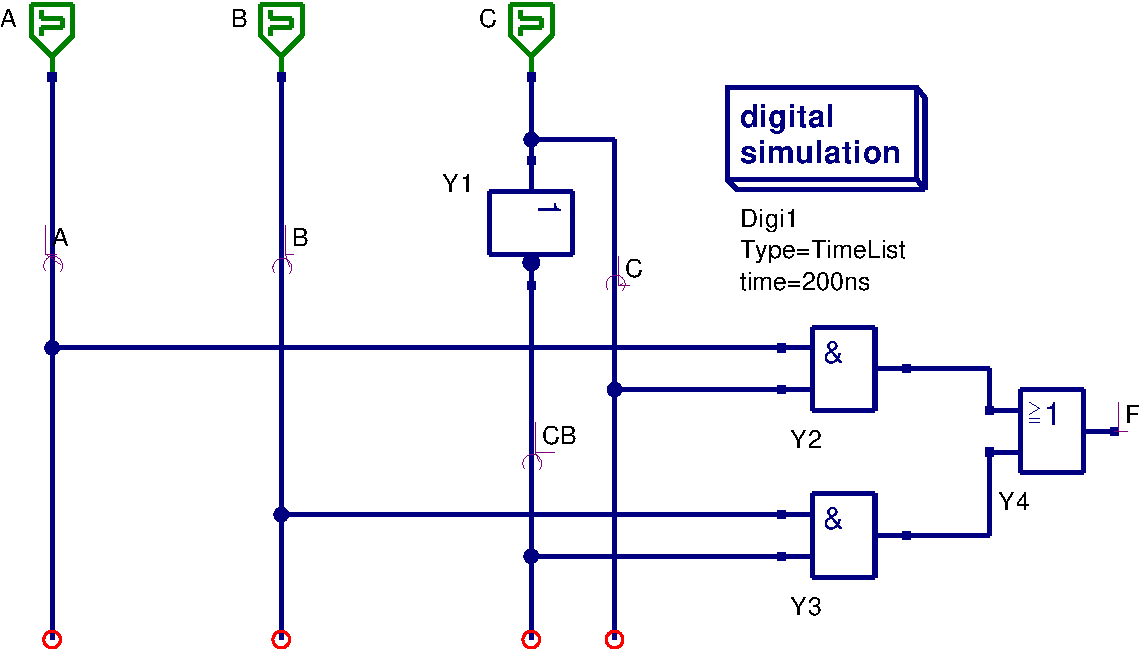
\includegraphics[width=0.9\linewidth]{dtut1}
  \caption{Qucs schematic for minimised logic function F}
  \label{fig:dtut1}
\end{figure} 
\FloatBarrier

\tutsection{VHDL code generated by Qucs}

Clicking the Qucs Simulate menu button (or pressing key F2) starts the
simulation process. At an early phase in this process Qucs writes a
text file to disk that contains the VHDL code for the circuit being
simulated.  This file can be displayed by clicking on the
\textit{\textbf{show last netlist}} drop down menu or by pressing key
F6. The VHDL code produced by Qucs for the circuit shown in
Fig.~\ref{fig:dtut1} is presented in Table~\ref{tab:tab2}.

\begin{table}
\begin{lstlisting}[language=VHDL]
-- Qucs 0.0.9  tut1_ex1.sch
entity TestBench is
end entity;
use work.all;

architecture Arch_TestBench of TestBench is
signal CB, A,  B,  F, C, 
       nnnet0, 
       nnnet1 : bit;
begin
  nnnet0 <= C and A;
  nnnet1 <= CB and B;
  CB <= not C;

  A:process
  begin
    A <= '0';  wait for 40 ns;
    A <= '1';  wait for 40 ns;
  end process;


  B:process
  begin
    B <= '0';  wait for 20 ns;
    B <= '1';  wait for 20 ns;
  end process;

  F <= nnnet1 or nnnet0;

  C:process
  begin
    C <= '0';  wait for 10 ns;
    C <= '1';  wait for 10 ns;
  end process;

end architecture;
\end{lstlisting}
\caption{VHDL code for the circuit shown in Fig.~\ref{fig:dtut1}}
\label{tab:tab2}
\end{table}
\FloatBarrier

Signals identified by nnnet0 and nnnet1 in Table~\ref{tab:tab2} have
been allocated these names by Qucs; nnnet0 and nnnet1 are internal
signal nets that are not named on the circuit schematic shown in
Fig.~\ref{fig:dtut1}.  Fig.~\ref{fig:tdex1} illustrates the starting
section of a typical Qucs digital functional waveform plot.  This
style of plot illustrates signal events without component delays.  If
required, signal delays can be specified for individual gates and
other components (from the component \textbf{\textit{edit properties}}
menu).  The VHDL code generated for components with delays will then
reflect such changes, for example adding a 10 ns delay to signal CB in
Table~\ref{tab:tab2} generates VHDL code
\begin{lstlisting}[language=VHDL]
CB <= not C after 10 ns;
\end{lstlisting}

Readers will probably have observed that the Qucs version number
referred to in Table~\ref{tab:tab2} VHDL listing is 0.0.9.  This is
the current CVS development version number.  Qucs 0.0.9 includes a
number of important bug fixes.  The remainder of these notes assume
readers have downloaded, and recompiled, the latest CVS code from
Sourceforge.net\footnote{Please note, Qucs Linux release 0.0.8 will
normally simulate single hierarchy digital circuits without error.
However, Qucs 0.0.8 does fail at the VHDL to C++ conversion phase if a
schematic includes more than one ground symbol.}.

\begin{figure}[ht]
  \centering
  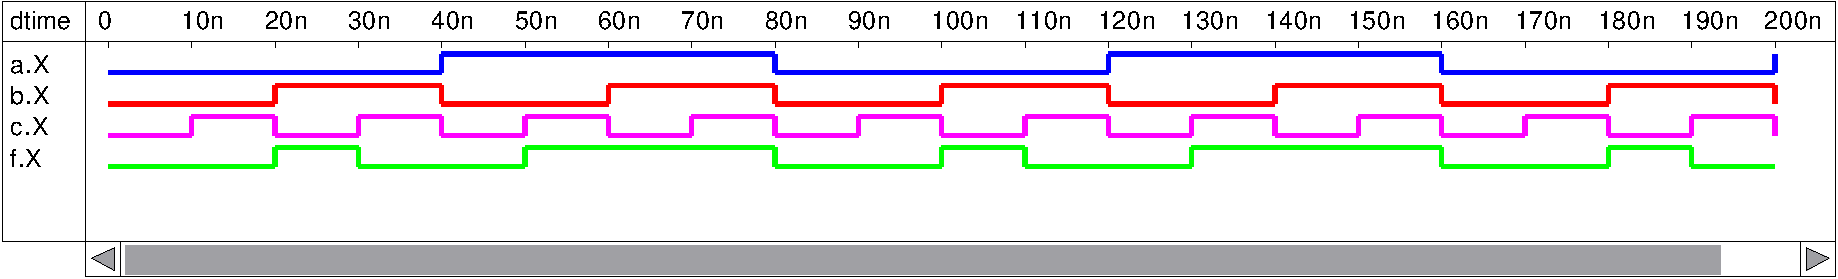
\includegraphics[width=1\linewidth]{tdex1}
  \caption{Digital functional waveforms for the circuit shown in Fig.~\ref{fig:dtut1}}
  \label{fig:tdex1}
\end{figure}
\FloatBarrier

\tutsection{Truth tables}

Truth tables are one of the most fundamental and convenient ways of
displaying digital circuit data.  Qucs has a built-in facility that
allows a truth table to be generated from a schematic drawing.  This
feature is particularly useful when checking minimised logic designs
for errors.  Lets consider a simple but instructive example: A logic
circuit has four binary inputs A, B, C, and D, and one output P.
Output P is logic '1' when inputs ABCD are prime numbers.  The four
binary inputs have numbers in the range "0000" to "1111" (0 to 15 in
decimal) with prime numbers 1, 3, 5, 7, 11 and 13.  In Boolean sum of
product form \\
\begin{center}
\begin{large}$F=\overline{A}.\overline{B}.\overline{C}.D+\overline{A}.\overline{B}.C.D+
\overline{A}.B.\overline{C}.D+\overline{A}.B.C.D+A.\overline{B}.C.D$
\end{large}\end{center}

This simplifies to\\
\begin{center}
\begin{large}$P=D.(A+B \oplus C )$\end{large}
\end{center}
The schematic for the sum of products equation for P is shown in
Fig.~\ref{fig:prim1sch}.  Similarly Fig.~\ref{fig:prim2sch} presents
the schematic for a minimised P equation.  Setting the digital
simulation type to TruthTable, rather than TimeList, causes Qucs on
pressing key F2, to generate a truth table based on the information
provided on a circuit schematic. The number of truth table inputs, and
indeed outputs, correspond to the number of input generators and the
number of named outputs. Truth tables for both schematics are given in
Table~\ref{tab:prim1tt} and~\ref{tab:prim2tt}. Comparing these two
tables clearly indicates that they are not identical and moreover
confirms that the minimised solution is not correct.  Reworking the
minimisation procedure points to the error being a missing signal
inversion.  The correct Boolean equation for P is

\begin{center}
\begin{large}$P=D.(\overline{A}+B \oplus C )$\end{large}
\end{center}

\begin{figure}
  \centering
\subfigure[Schematic diagram for sum of products equation P]{
  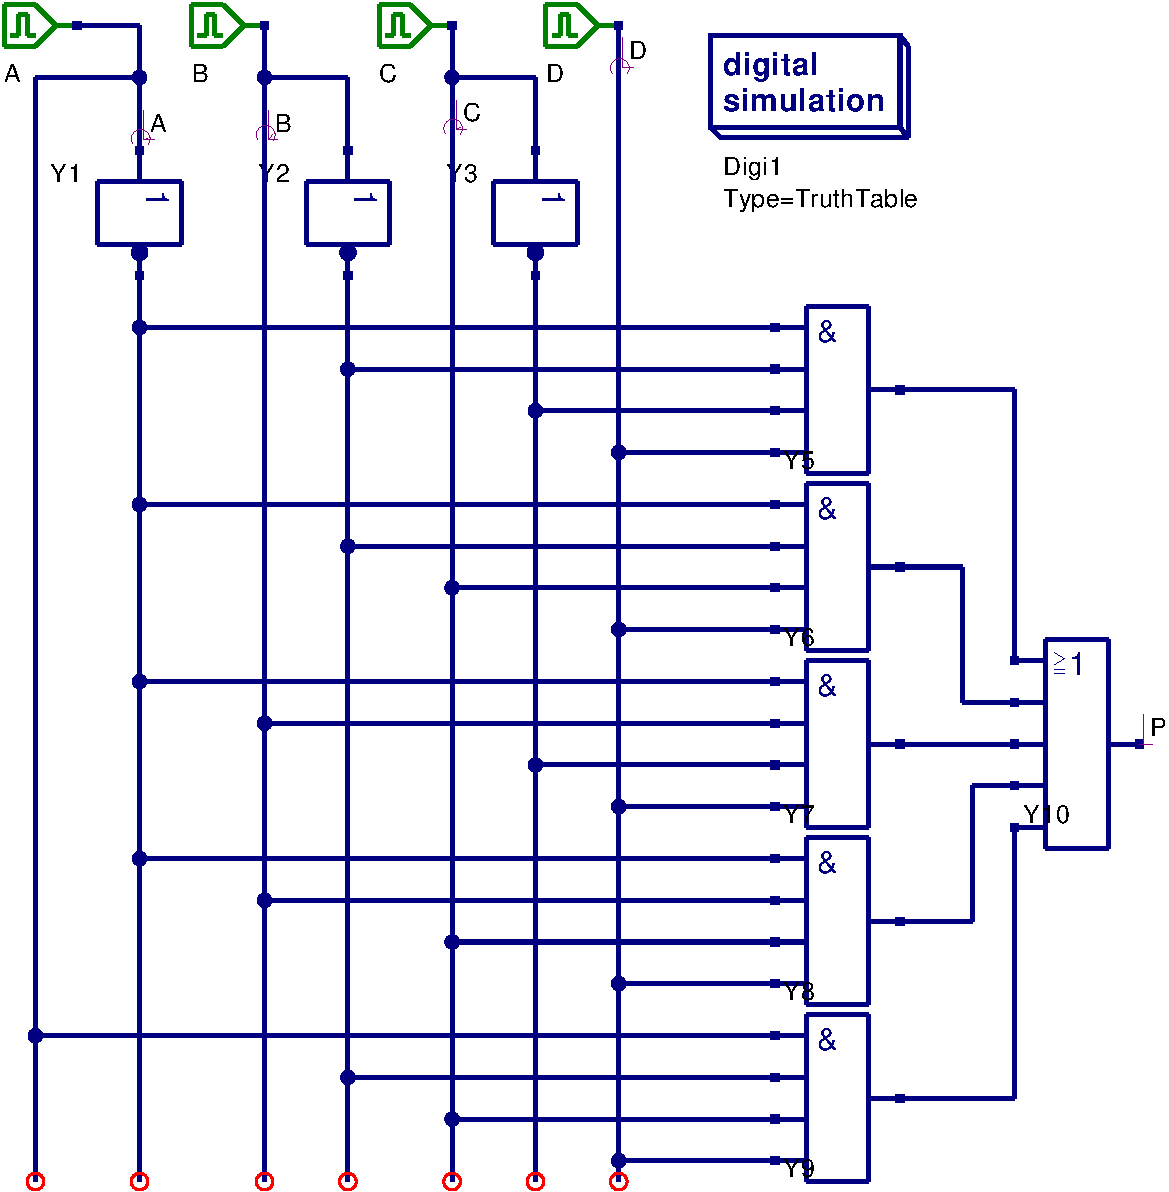
\includegraphics[width=.7\linewidth]{prim1sch}
  \label{fig:prim1sch}}
% prim1sch.png: 99.9998dpi, width=8.15cm, height=8.31cm, bb=0 0 321 327
\subfigure[Schematic diagram for minimised equation P]{
  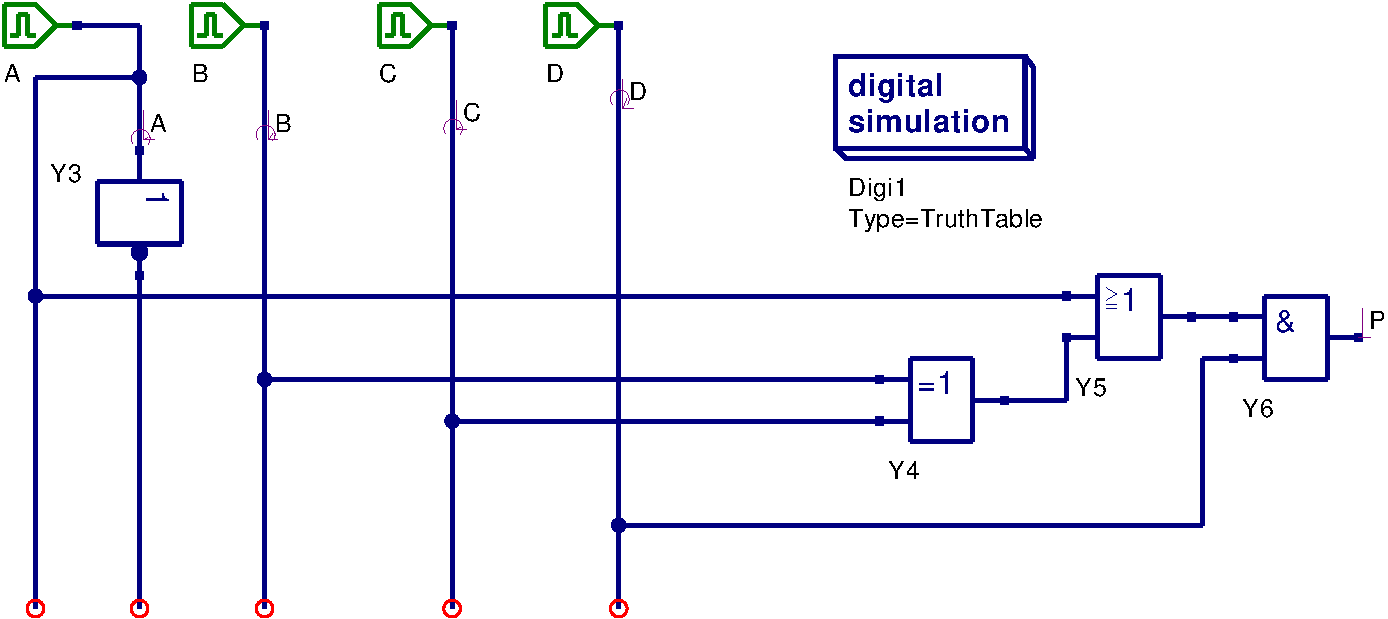
\includegraphics[width=.9\linewidth]{prim2sch}
  \label{fig:prim2sch}}
% prim1sch.png: 99.9998dpi, width=10.21cm, height=4.62cm, bb=0 0 402 182
\end{figure}
\FloatBarrier

\begin{table}
  \centering
\subtable[Truth table for sum of products equation P]{
  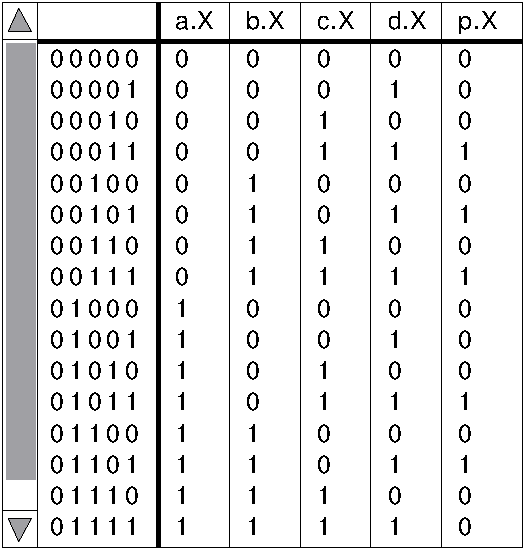
\includegraphics[width=.4\linewidth]{prim1tt}
% prim1tt.png: 200dpi, width=1.91cm, height=1.91cm, bb=0 0 150 150
  \label{tab:prim1tt}}
\\
\subtable[Truth table for minimised equation P]{
  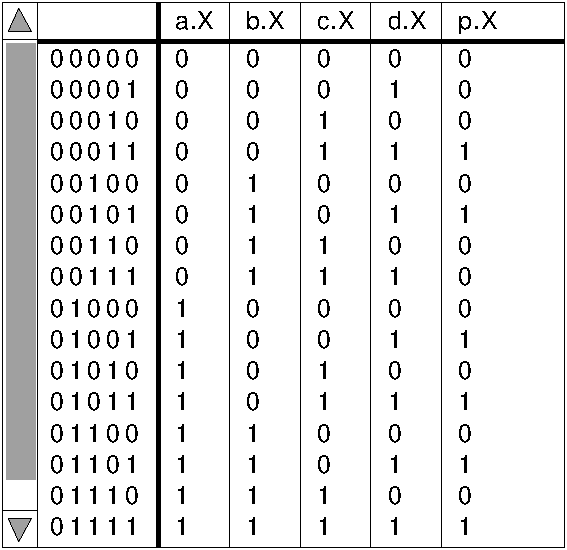
\includegraphics[width=.435\linewidth]{prim2tt}
  \label{tab:prim2tt}}
% prim2tt.png: 99.9998dpi, width=3.94cm, height=3.91cm, bb=0 0 155 154
\end{table}
\FloatBarrier

\tutsection{Digital subcircuits}

Although it is possible to draw complex schematic diagrams using only
the predefined digital components supplied with Qucs, this technique
can be extremely tedious, and is of course, prone to error.  When
drawing large schematics we require a design procedure that naturally
subdivides groups of digital components into self contained units.
These units can then be treated in the same way as basic digital
components when placing and connecting them on a schematic drawing.
In the world of analogue and digital circuit design such units are
often called subcircuits.\footnote{The circuit simulator SPICE is a
well known example of a widely used CAD program that makes extensive
use of subcircuits in circuit design.}  A subcircuit is defined by
three major attributes plus a number of other properties. The major
attributes are, firstly a digital circuit that defines circuit
function, secondly a circuit symbol that depicts a circuit in a higher
level of a design hierarchy, and thirdly the subcircuit input/output
pins shown on the subcircuit symbol.  Other properties include for
example, signal path delays. The process for generating digital
subcircuits is identical to that used for analogue subcircuits.  It is
best demonstrated by considering an example.
Figure~\ref{fig:t1ex2sch} shows the schematic for a four input
combinational circuit.

\begin{figure}
  \stepcounter{figure}
  \centering
  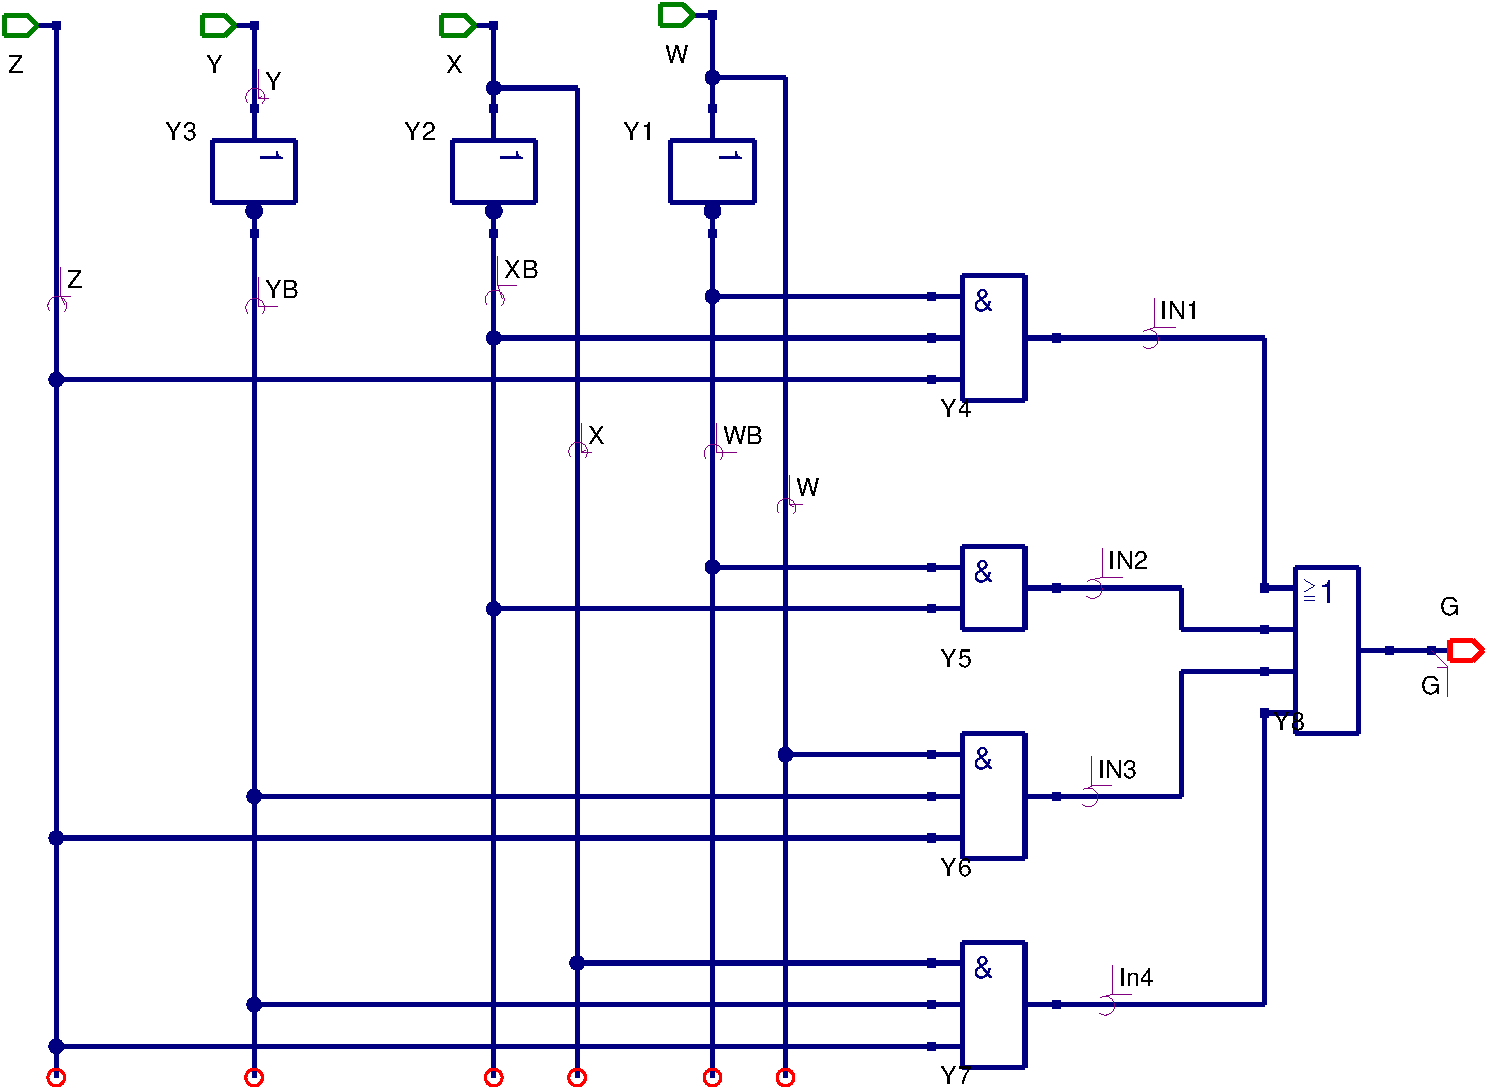
\includegraphics[width=0.8\linewidth]{t1ex2sch}
% tcomb1.png: 99.9998dpi, width=11.35cm, height=3.35cm, bb=0 0 447 132
  \caption{Combinational logic circuit with inputs W, X, Y, Z, and output G}
  \label{fig:t1ex2sch}
\end{figure}
\FloatBarrier

After drawing a subcircuit schematic, input and output\footnote{Qucs
  0.0.8 has a bug which causes a VHDL compile error when subcircuit
  pins are specified as type out. A work around for this bug is to
  specify subcircuit output pins as type analog.  The Qucs routines
  that generate the circuit VHDL code convert pin type analog into
  VHDL type inout. FreeHDL is then able to compile the generated VHDL
  code without error. This bug has been corrected in Qucs 0.0.9} pins
are attached to signal ports.  Input port pins of type in are shown on
circuit diagrams as a green symbol, signals W, X, Y, and Z, in
Fig.~\ref{fig:t1ex2sch}.  Ouput port pins of type out are coloured
red, signal G in Fig.~\ref{fig:t1ex2sch}. Signal flow through a port
is indicated by the direction of the port symbol arrow
head. Input/output signals, and any other signals that need to be
easily identified, are also named.  Once the subcircuit schematic is
complete, pressing key F3 causes Qucs to generate a subcircuit symbol.
The drawing tools listed as icons in the Qucs paintings window can be
used to edit Qucs generated subcircuit symbols.  The input/output port
pins on a subcircuit symbol have the same type and name as those on
the original subcircuit schematic.  Fig.~\ref{fig:comb1s} shows the
finished symbol for subcircuit COMB1. In these notes, symbol outlines
are shown drawn in accordance with the international code for logic
symbols\footnote{Ian, Kampel, A practical introduction to the new
  logic symbols, Butterworths, 1985, ISBN 0-408-01461-X}. To test our
new subcircuit we place it's symbol on a blank drawing sheet and apply
test signals to the input pins and observe the signals at the output
pin.  Fig.~\ref{fig:tcomb1s} shows a typical test circuit.  Subcircuit
Gen4bit generates a 4 bit test pattern synchronised to the input of a
digital clock. The specification for Gen4bit is given in the next
section of these notes\footnote{Subcircuit Gen4bit includes other
  nested subcircuits.  Qucs 0.0.8 has a bug that causes VHDL compile
  errors with some configurations of nested subcircuits. This has been
  fixed in version 0.0.9 }.  The test pattern waveform and output
signal G are shown plotted as a function of time in
Fig.~\ref{fig:tcomb1}.

\begin{figure}
  \centering
  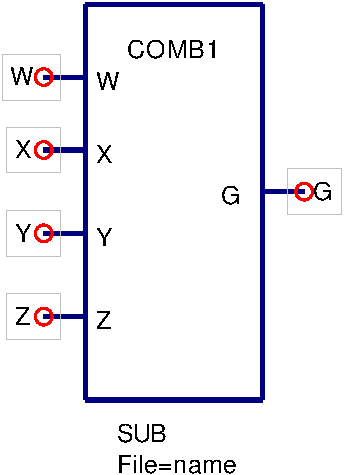
\includegraphics[width=0.2\linewidth]{comb1s}
% comb1s.png: 399.999dpi, width=2.72cm, height=3.92cm, bb=0 0 428 617
  \caption{Qucs symbol for a logic circuit with inputs W, X, Y, Z, and output G}
  \label{fig:comb1s}
\end{figure}
\FloatBarrier

\begin{figure}
  \centering
  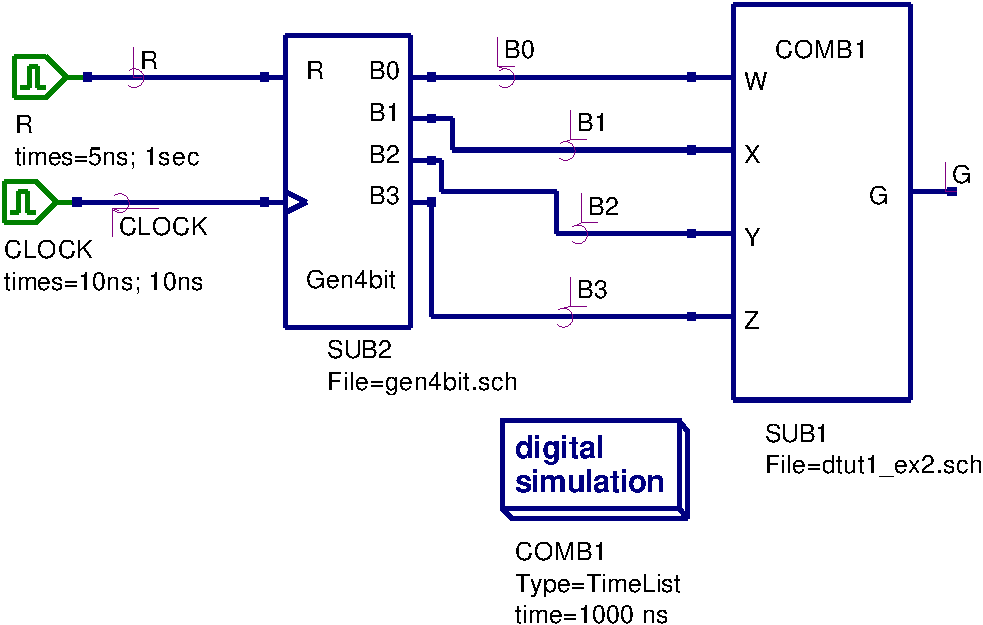
\includegraphics[width=0.8\linewidth]{tcomb1s}
% tcomb1s.png: 399.999dpi, width=7.44cm, height=4.72cm, bb=0 0 1172 743
  \caption{Test schematic for a logic circuit with inputs W, X, Y, Z, and output G}
  \label{fig:tcomb1s}
\end{figure}
\FloatBarrier

\begin{figure}
  \centering
  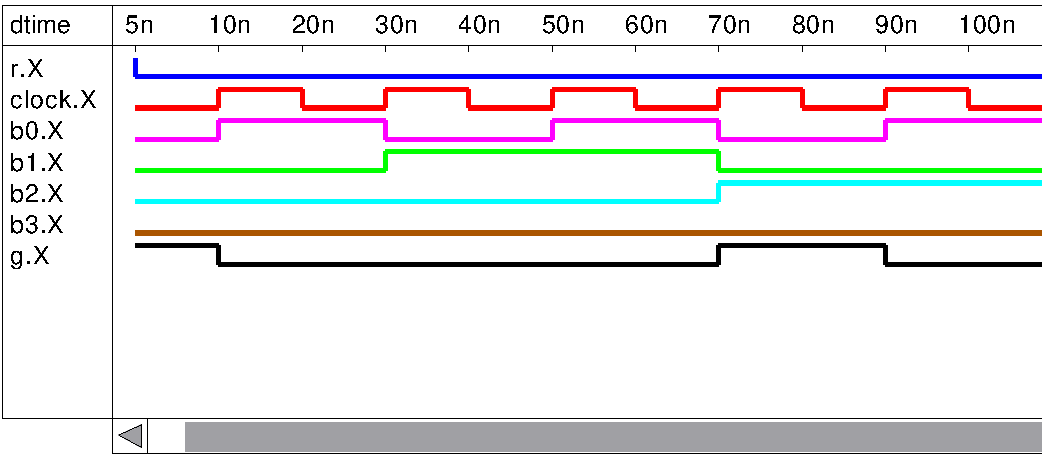
\includegraphics[width=0.9\linewidth]{tcomb1}
% tcomb1w.png: 399.999dpi, width=7.94cm, height=3.24cm, bb=0 0 1250 510
  \caption{Digital functional waveforms for a logic circuit with inputs W, X, Y, Z, and output G}
  \label{fig:tcomb1}
\end{figure}
\FloatBarrier

\tutsection{Building a digital component library}

The Qucs graphical user interface includes good project handling
features.  Combining these features with the Qucs subcircuit
capabilities provides all the tools required for the development of a
library of common digital components.  Such a library can be stored in
a master project and the individual component files imported into
other projects when required.  Here are a few components that I
developed during a recent series of tests aimed at detecting bugs in
the VHDL code generated by Qucs.

\tutsubsection{Logic zero}

\begin{flushleft}
  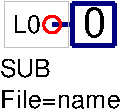
\includegraphics[width=.13\linewidth]{lzero} \hspace{10mm} 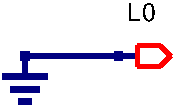
\includegraphics[width=0.23\linewidth]{lzerosch}
% lzerosch.png: 99.9998dpi, width=3.15cm, height=1.27cm, bb=0 0 124 50

% lzero.png: 99.9998dpi, width=1.50cm, height=1.45cm, bb=0 0 59 57
\end{flushleft}

\tutsubsection{Logic one}

\begin{flushleft}
  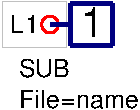
\includegraphics[width=.13\linewidth]{lone} \hspace{10mm} 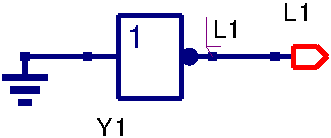
\includegraphics[width=0.23\linewidth]{lonesch}
% lonesch.png: 99.9998dpi, width=3.33cm, height=1.42cm, bb=0 0 131 56
\end{flushleft}

\tutsubsection{G2bit - 2 bit pattern generator}

\begin{center}
  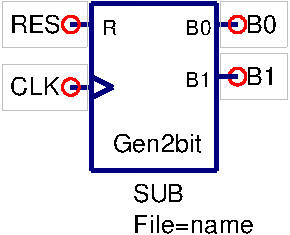
\includegraphics[]{g2bit}  
  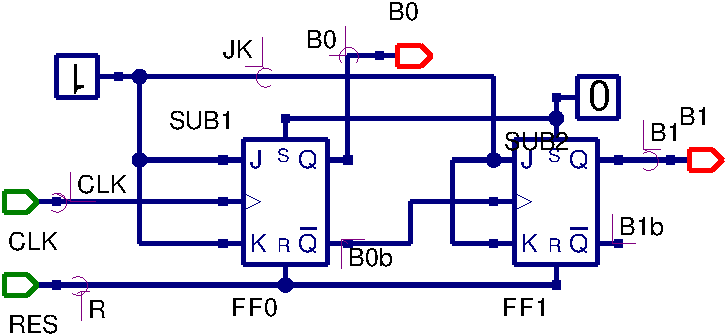
\includegraphics[width=0.8\linewidth]{g2bitsch}
\end{center}

\tutsubsection{G4bit - 4 bit pattern generator}

\begin{center}
  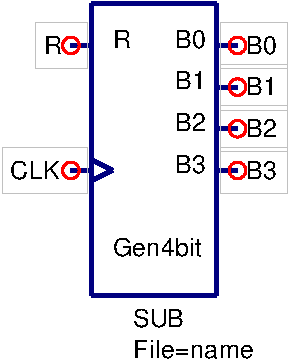
\includegraphics[]{g4bit}    
  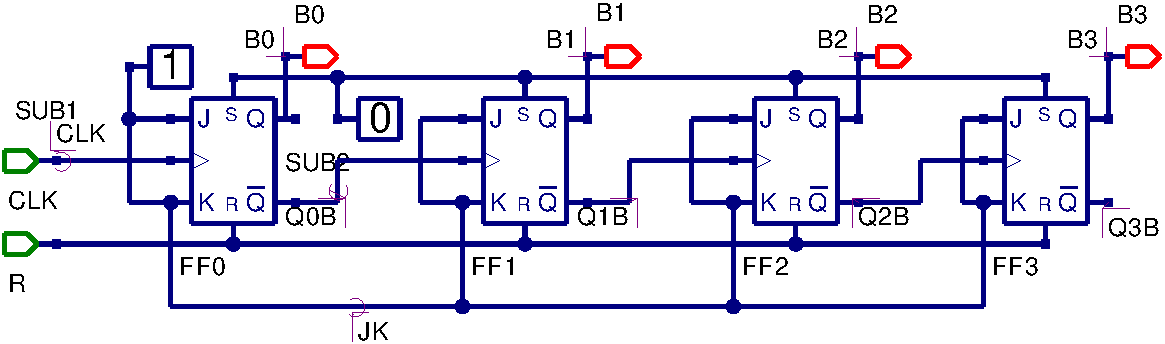
\includegraphics[width=1\linewidth]{g4bitsch}
% g4bit.png: 99.9998dpi, width=8.26cm, height=11.68cm, bb=0 0 325 460
\end{center}

\tutsubsection{MUX2to1 - 2 input to 1 output multiplexer}

\begin{center}
\begin{tabular}{lll}
EN & A & Y \\  
1 & X & L \\ 
0 & 0 & D0 \\ 
0 & 1 & D1
\end{tabular} 
\end{center}

\begin{center}
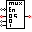
\includegraphics[]{mux2to1}
% mux2to1.png: 99.9998dpi, width=2.69cm, height=3.33cm, bb=0 0 106 131
\end{center}
\vspace{10mm}
\begin{center}
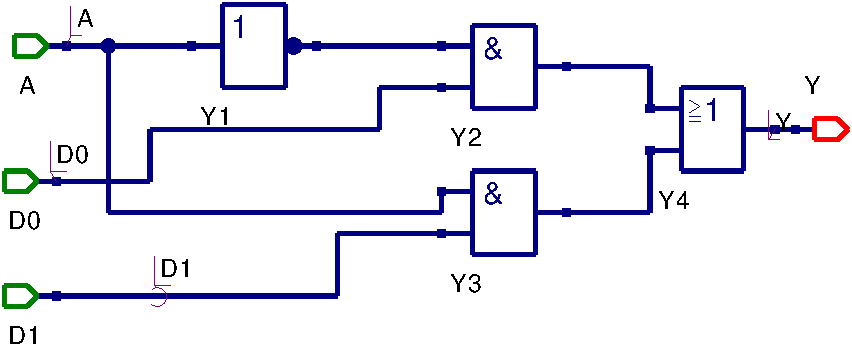
\includegraphics[]{mux2to1sch}
% mux2to1sch.png: 99.9998dpi, width=7.87cm, height=4.09cm, bb=0 0 310 161
\end{center}

\tutsubsection{MUX4to1 - 4 input to 1 multiplexer}

\vspace{5mm}
\begin{center}
\begin{tabular}{llll}
B & A & EN & Y \\ 
X & X & 1 & 0 \\ 
0 & 0 & 0 & D0 \\ 
0 & 1 & 0 & D1 \\ 
1 & 0 & 0 & D2 \\ 
1 & 1 & 0 & D3
\end{tabular}
\end{center}
\vspace{2mm}
\begin{center}
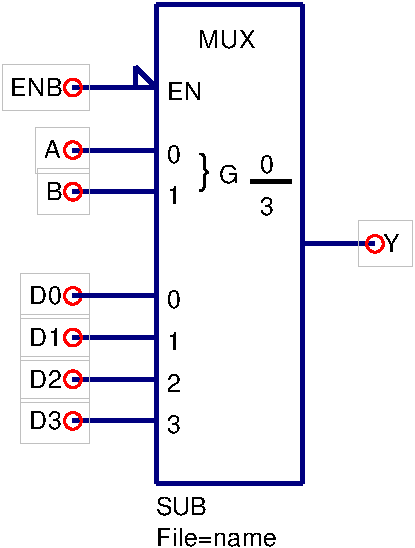
\includegraphics[width=0.3\linewidth]{mux4to1}
% mux4to1.png: 99.9998dpi, width=2.79cm, height=4.19cm, bb=0 0 110 165
\end{center}
\begin{center}
  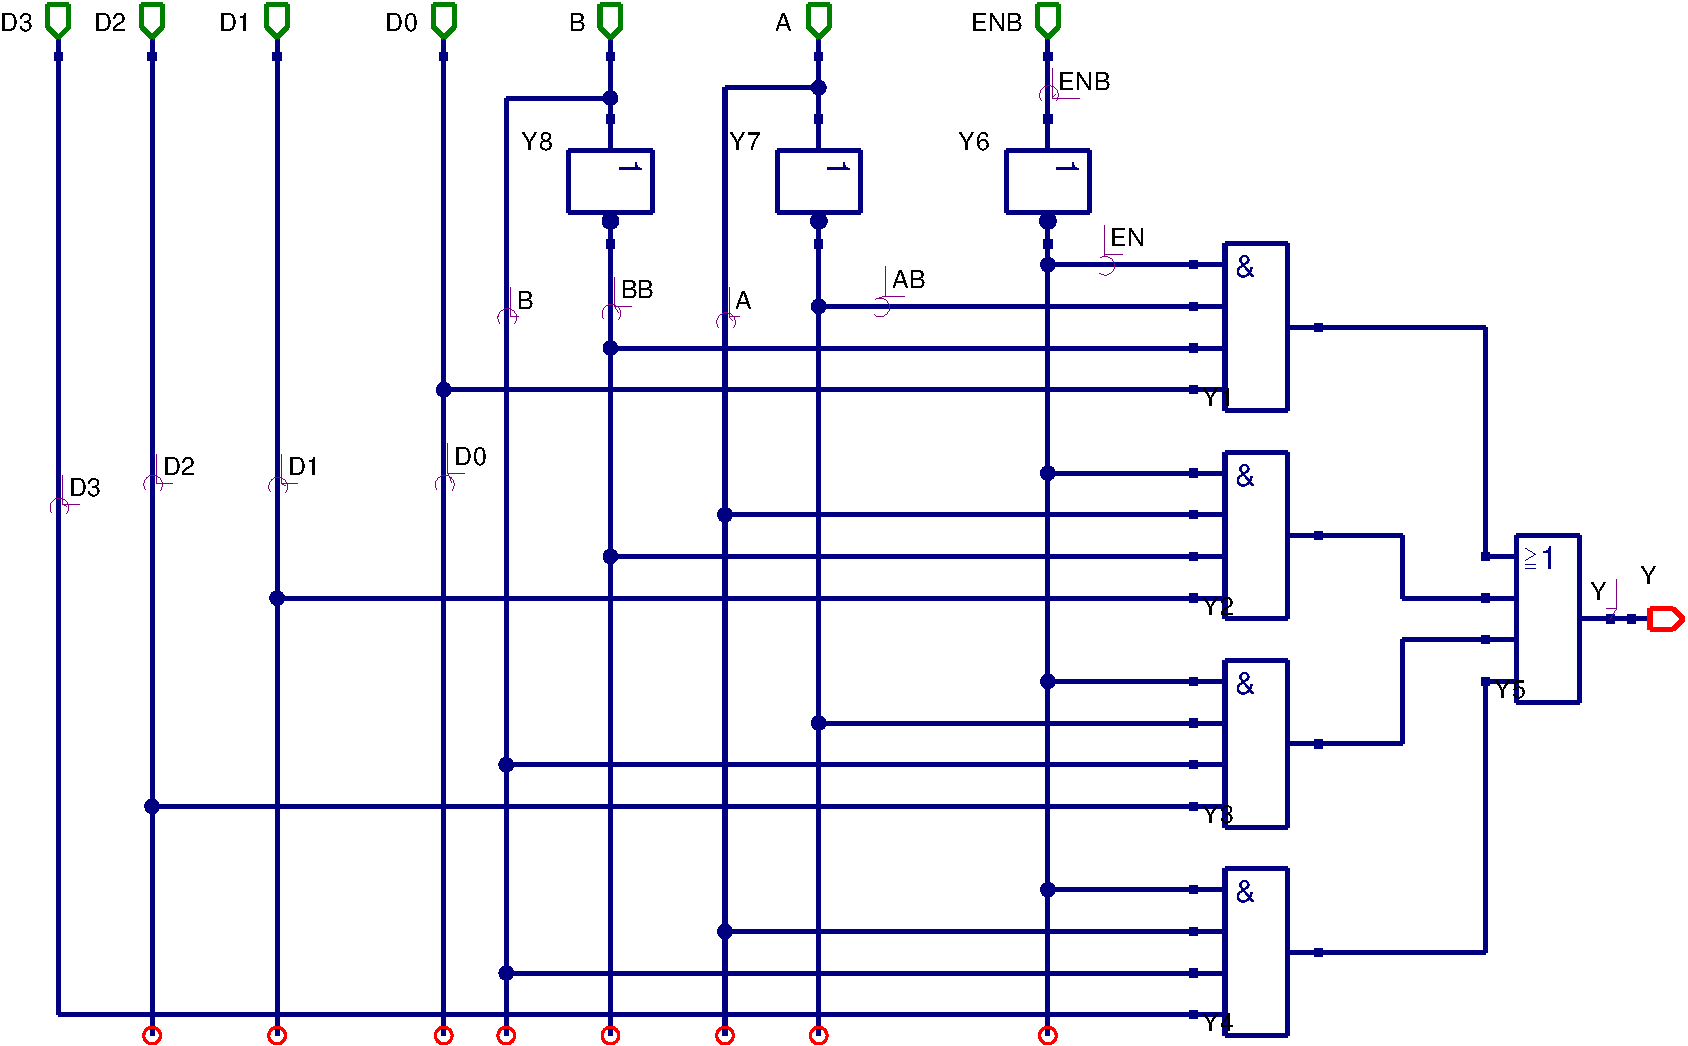
\includegraphics[width=1\linewidth]{mux4to1sch}
% mux4to1sch.png: 99.9998dpi, width=11.40cm, height=7.44cm, bb=0 0 449 293
\end{center}

\tutsubsection{2 bit adder}

\begin{center}
  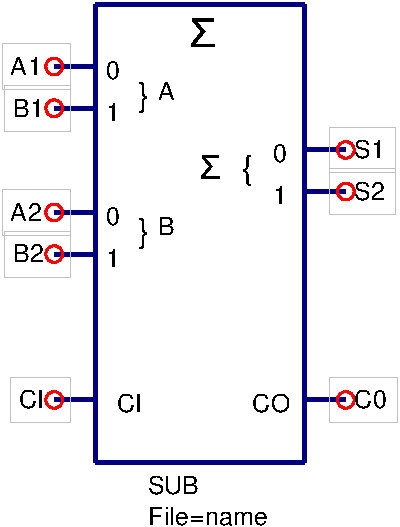
\includegraphics[width=0.3\linewidth]{fadder2bit}
% fadder2bit.png: 99.9998dpi, width=3.28cm, height=4.19cm, bb=0 0 129 165
\end{center}
\begin{center}
  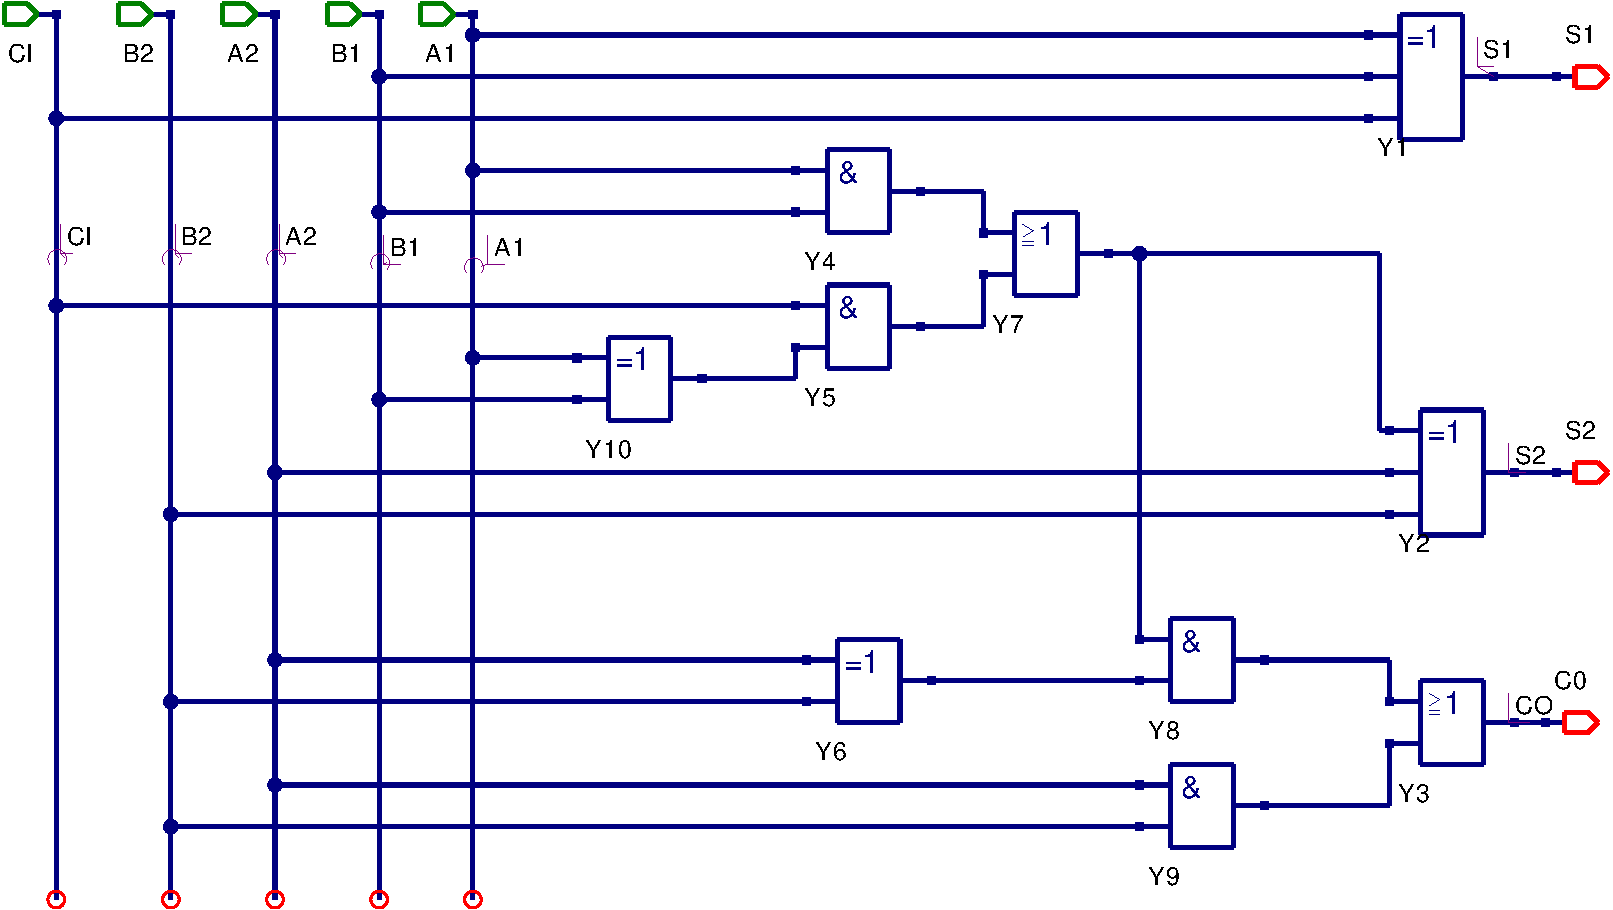
\includegraphics[width=1\linewidth]{fadder2bitsch}
% fadder2bitsch.png: 99.9998dpi, width=11.23cm, height=6.88cm, bb=0 0 442 271
\end{center}

\tutsection{Subcircuit VHDL code generated by Qucs}

Qucs generates a separate entity-architecture model for each
subcircuit.  These component definitions are compiled into the work
library by FreeHDL.  Here is the VHDL code from two of the previous
examples.

\tutsubsection{Gen2bit}
\begin{lstlisting}[language=VHDL]
entity Sub_gen2bit is
  port (CLK: in bit;
        R: in bit;
        nnout_B0: out bit;
        nnout_B1: out bit);
end entity;
use work.all;
architecture Arch_Sub_gen2bit of Sub_gen2bit is
  signal B0b,
         B1b,
         JK,
         nnnet0,
         B0,
         B1 : bit;
begin
  FF0 : process (nnnet0, R, CLK)
  begin
    if (R='1') then  B0 <= '0';
    elsif (nnnet0='1') then  B0 <= '1';
    elsif (CLK='1' and CLK'event) then
      B0 <= (JK and not B0) or (not JK and B0);
    end if;
  end process;
  B0b <= not B0;

  FF1 : process (nnnet0, R, B0b)
  begin
    if (R='1') then  B1 <= '0';
    elsif (nnnet0='1') then  B1 <= '1';
    elsif (B0b='1' and B0b'event) then
      B1 <= (JK and not B1) or (not JK and B1);
    end if;
  end process;
  B1b <= not B1;

  SUB2: entity Sub_logic_zero port map (nnnet0);
  nnout_B0 <= B0 or '0';
  nnout_B1 <= B1 or '0';
  SUB1: entity Sub_Logic_one port map (JK);
end architecture;
\end{lstlisting}

\tutsubsection{2 bit adder}

\begin{lstlisting}[language=VHDL]
entity Sub_fadd_2bit is
  port (A1: in bit;
        B1: in bit;
        A2: in bit;
        B2: in bit;
        CI: in bit;
        nnout_S1: out bit;
        nnout_S2: out bit;
        nnout_CO: out bit);
end entity;
use work.all;
architecture Arch_Sub_fadd_2bit of Sub_fadd_2bit is
  signal nnnet0,
         nnnet1,
         nnnet2,
         nnnet3,
         nnnet4,
         nnnet5,
         nnnet6,
         S2,
         CO,
         S1 : bit;
begin
  S1 <= CI xor B1 xor A1;
  nnnet0 <= B2 xor A2;
  nnnet1 <= nnnet0 and nnnet2;
  nnnet3 <= B2 and A2;
  nnnet2 <= nnnet4 or nnnet5;
  nnnet4 <= nnnet6 and CI;
  nnnet5 <= B1 and A1;
  S2 <= B2 xor A2 xor nnnet2;
  CO <= nnnet3 or nnnet1;
  nnnet6 <= B1 xor A1;
  nnout_S2 <= S2 or '0';
  nnout_CO <= CO or '0';
  nnout_S1 <= S1 or '0';
end architecture;
\end{lstlisting}

\tutsubsection{Notes on subcircuit VHDL generation}
\begin{itemize}
\item
Qucs predefined digital components generate concurrent data flow
signal statements or process statements.
\item
Previously defined subcircuit symbols generate VHDL port map
statements.
\item
 Type out entity port signals are prevented from being read as input
 signals by masking each output signal using the logic
 function:\linebreak signal-name OR '0'.\footnote{Attempting to read
 entity port signals of type out results in a VHDL compile error. }
\item
 A VHDL \begin{lstlisting}[language=VHDL]
use work.all; \end{lstlisting}
statement is included before each subcircuit architecture definition
to ensure that FreeHDL can find any nested subcircuits
\footnote{Strictly speaking it should not be necessary to specifically
state the use of the work library as this library is normally visible
at all times when compiling entity-architecture models.  However, at
this stage in the development of FreeHDL it does appear that it is
necessary when using the default FreeHDL VHDL library mapping.}.
\item
The complete VHDL code file for a digital design is composed from an
outer test bench entity-architecture model plus entity-architecture
models for each subcircuit specified in the design,
\end{itemize}

\tutsection{Subcircuit nesting: A more complex design example}

In theory there is no limit to the depth of subcircuit nesting allowed
by Qucs.  In practice most digital circuit schematics can be
constructed with a maximum of four or five levels of design hierarchy.
Figure~\ref{fig:regt} shows an example that was used to test Qucs
subcircuit nesting performance.  The design is a simple RTL function
that uses a multiplexer to transfer data from one of two input
registers to a single output register.  The next section of these
notes outlines in detail the specification of the subcircuits needed
to build the RTL design.  A set of sample simulation waveforms showing
the register transfer operation are illustrated in
Fig.~\ref{fig:testrtl}.

\tutsubsection{4 bit RTL design}

\begin{figure}[ht]
  \centering
  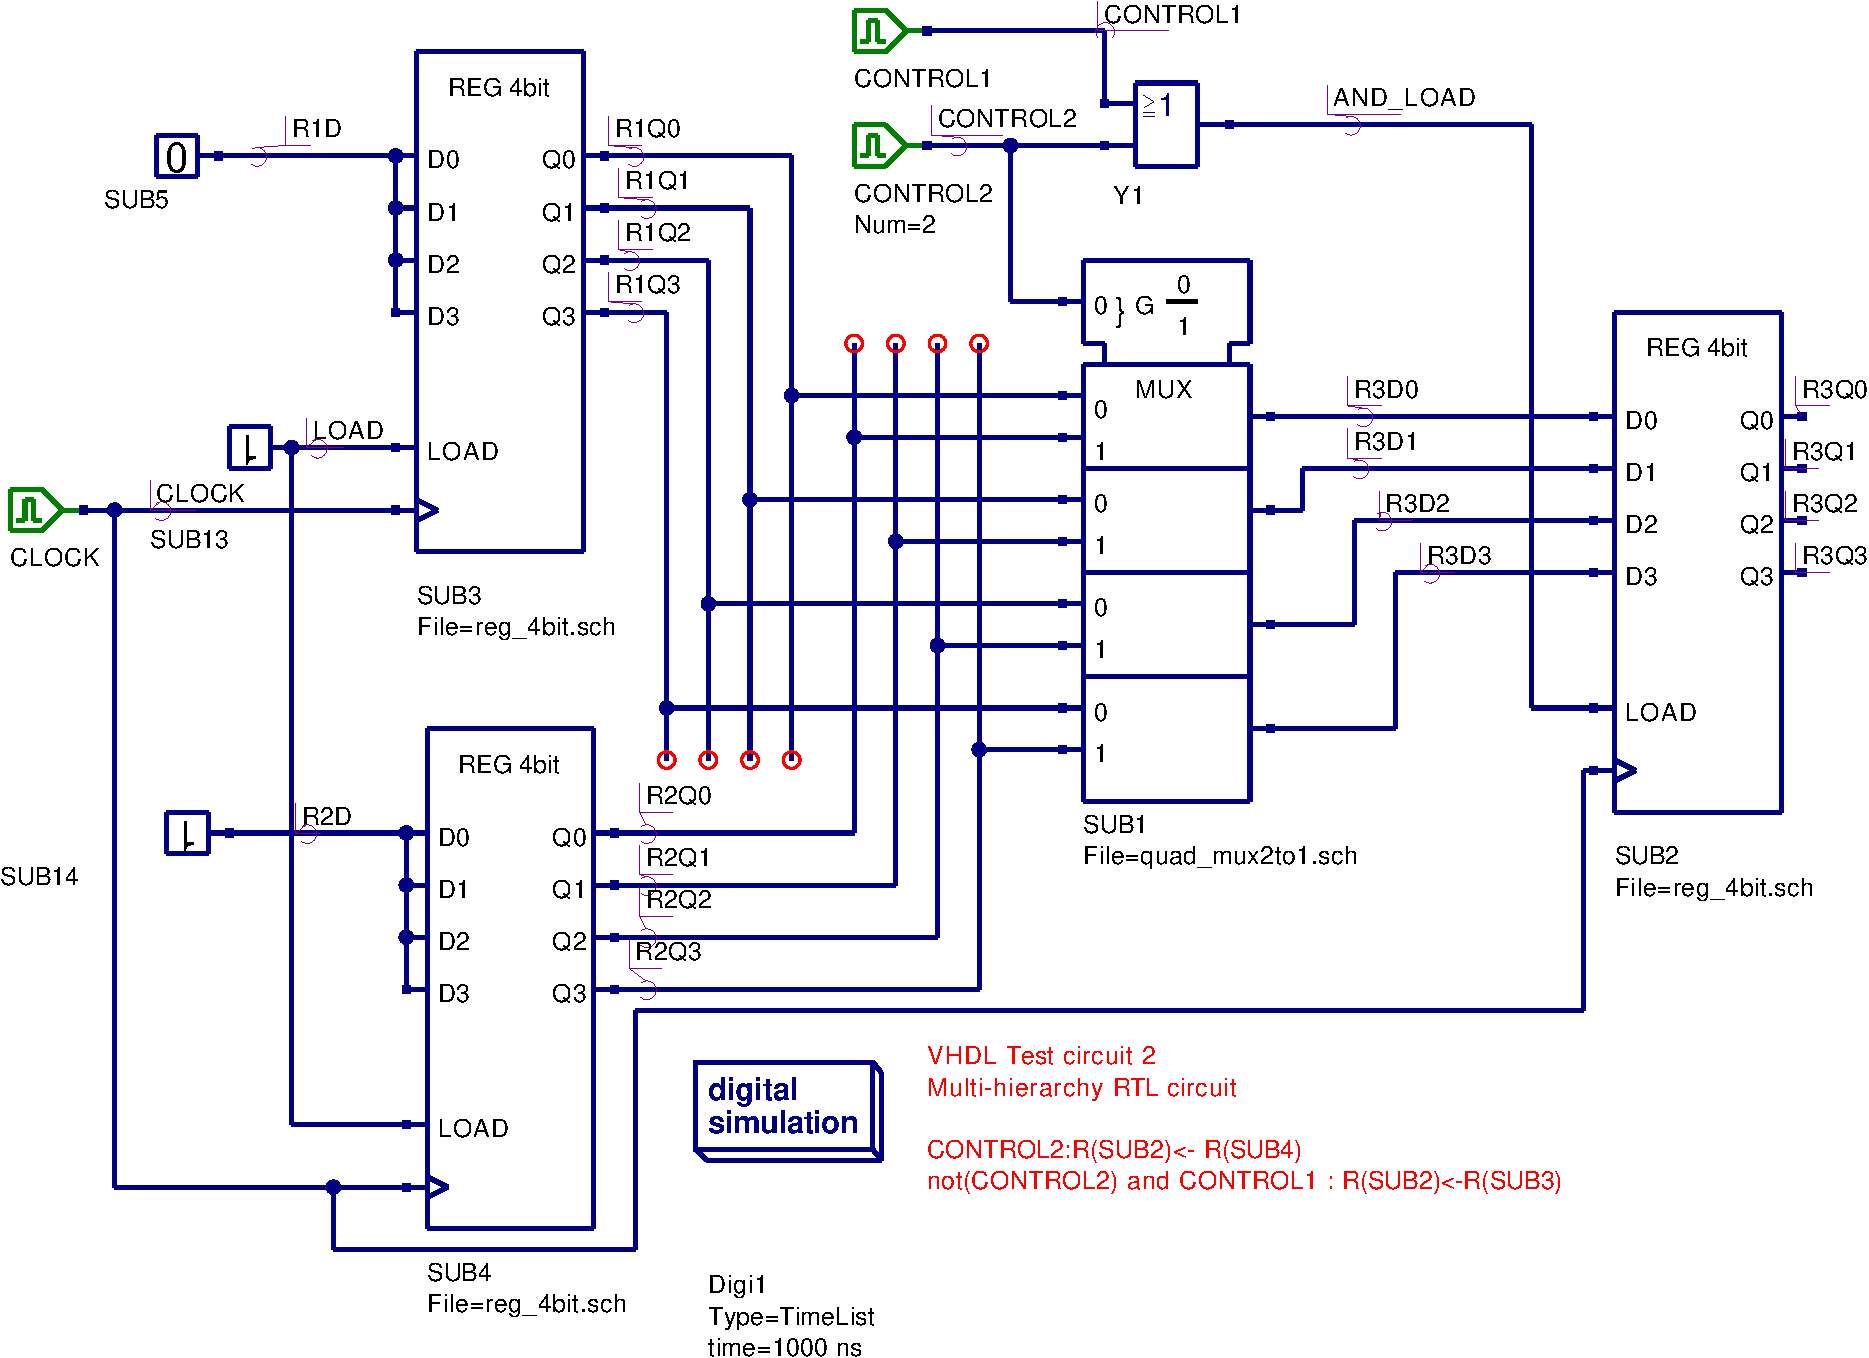
\includegraphics[width=1\linewidth]{regt}
% regt.png: 99.9998dpi, width=14.05cm, height=9.98cm, bb=0 0 553 393
  \caption{Top level schematic}
  \label{fig:regt}
\end{figure} 
\FloatBarrier

\tutsubsubsection{Reg4bit}

	\begin{center}
	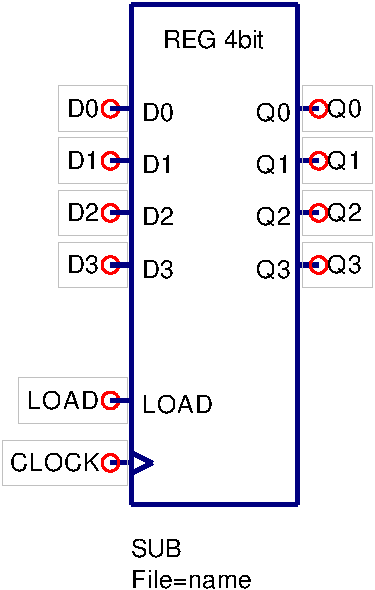
\includegraphics[width=.25\linewidth]{reg4bit}
% reg4bit.png: 99.9998dpi, width=2.69cm, height=4.32cm, bb=0 0 106 170
	\end{center}
\vspace{10mm}
	\begin{center}
	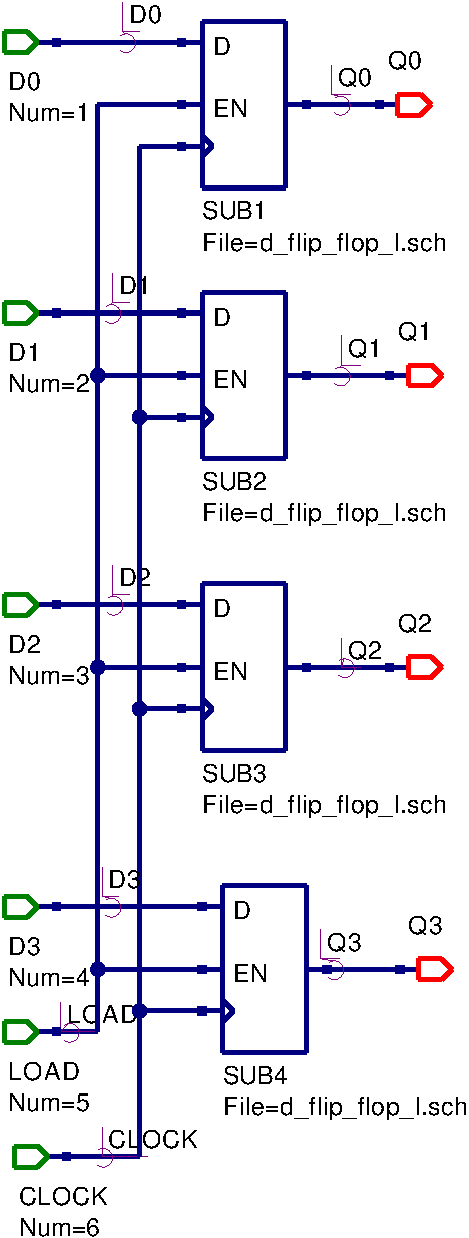
\includegraphics[width=.3\linewidth]{reg4bitsch}
% reg4bitsch.png: 99.9998dpi, width=6.38cm, height=13.72cm, bb=0 0 251 540
	\end{center}
\pagebreak
\tutsubsubsection{D flip-flop with load enable}
	\begin{center}
	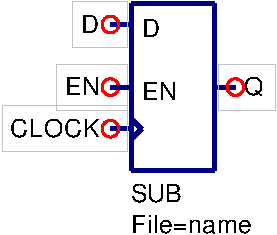
\includegraphics[width=0.2\linewidth]{dffl}
% dffl.png: 99.9998dpi, width=2.31cm, height=2.44cm, bb=0 0 91 96
	\end{center}

	\begin{center}
	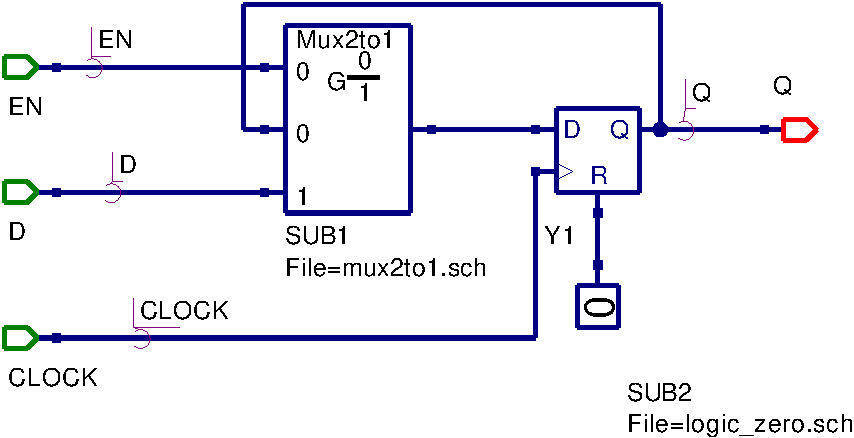
\includegraphics[width=0.7\linewidth]{dfflsch}
% dfflsch.png: 99.9998dpi, width=5.99cm, height=3.30cm, bb=0 0 236 130
	\end{center}
\tutsubsubsection{Mux2to1}
	\begin{center}
	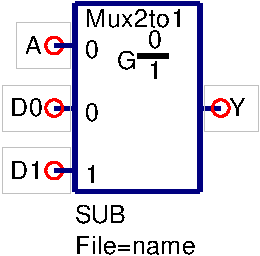
\includegraphics[width=0.2\linewidth]{mux21}
% mux21.png: 99.9998dpi, width=2.34cm, height=2.31cm, bb=0 0 92 91
	\end{center}
	\begin{center}
	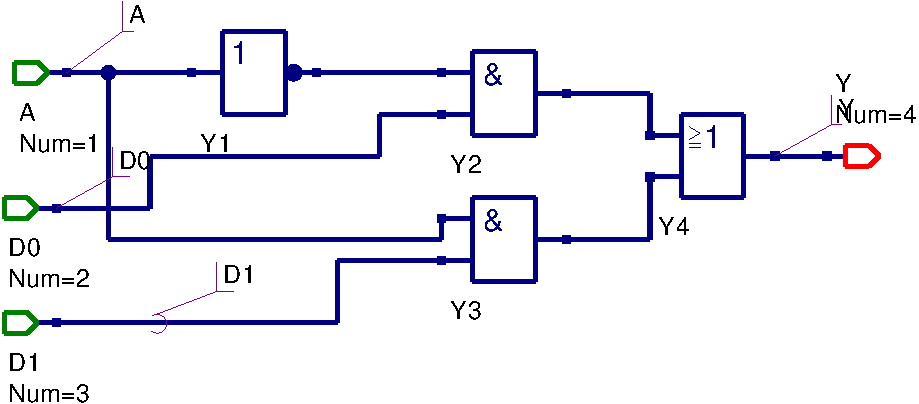
\includegraphics[width=0.7\linewidth]{mux21sch}
% mux21sch.png: 99.9998dpi, width=6.43cm, height=2.97cm, bb=0 0 253 117
	\end{center}
\tutsubsubsection{QuadMux}
	\begin{center}
	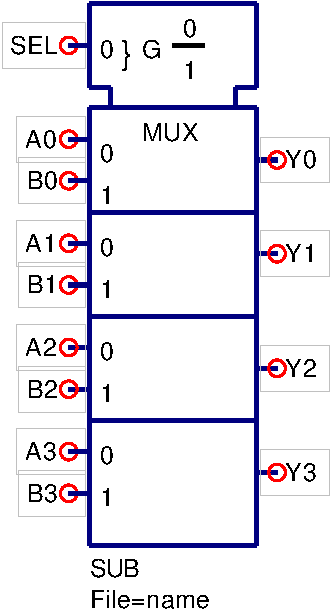
\includegraphics[width=0.2\linewidth]{quadmux}
% quadmux.png: 99.9998dpi, width=2.92cm, height=4.50cm, bb=0 0 115 177
	\end{center}
	\begin{center}
	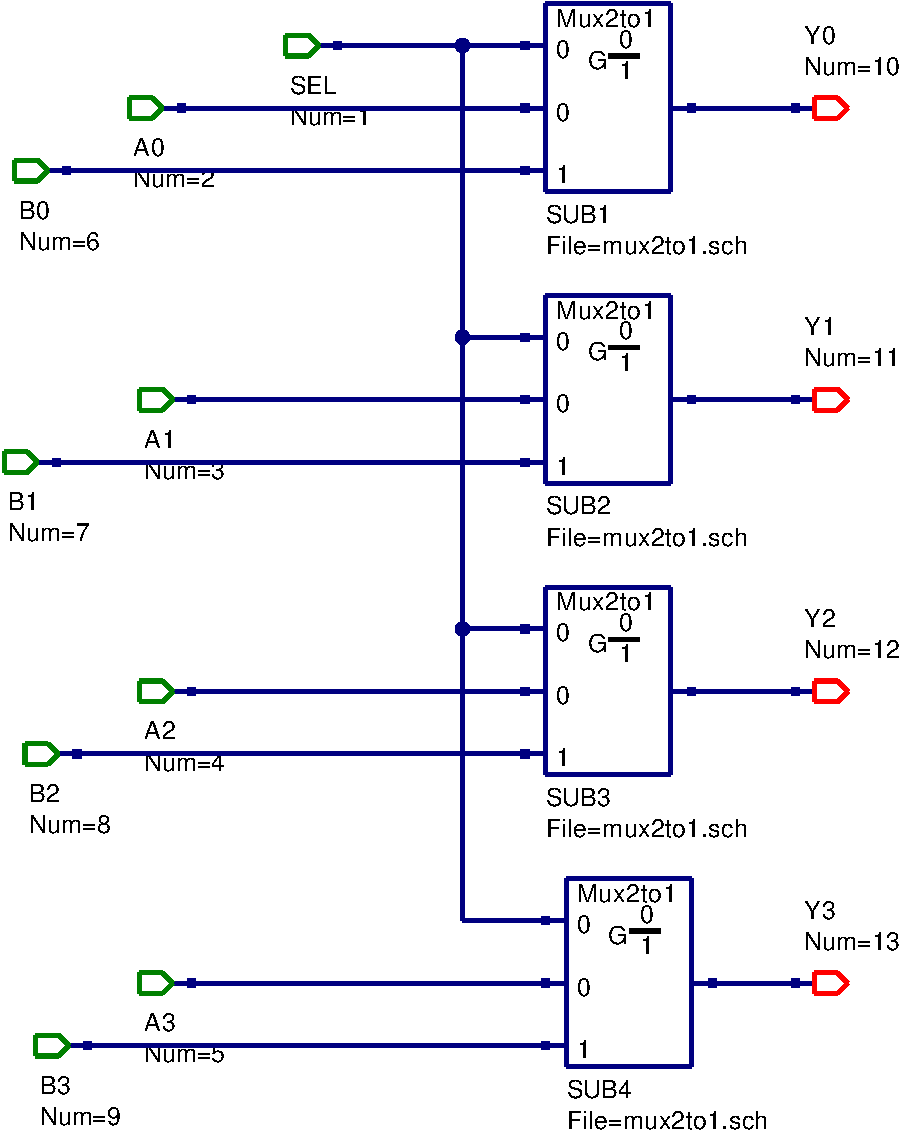
\includegraphics[width=0.7\linewidth]{quadmuxsch}
% quadmuxsch.png: 99.9998dpi, width=6.43cm, height=7.85cm, bb=0 0 253 309
	\end{center}

\begin{figure}[ht]
  \centering
  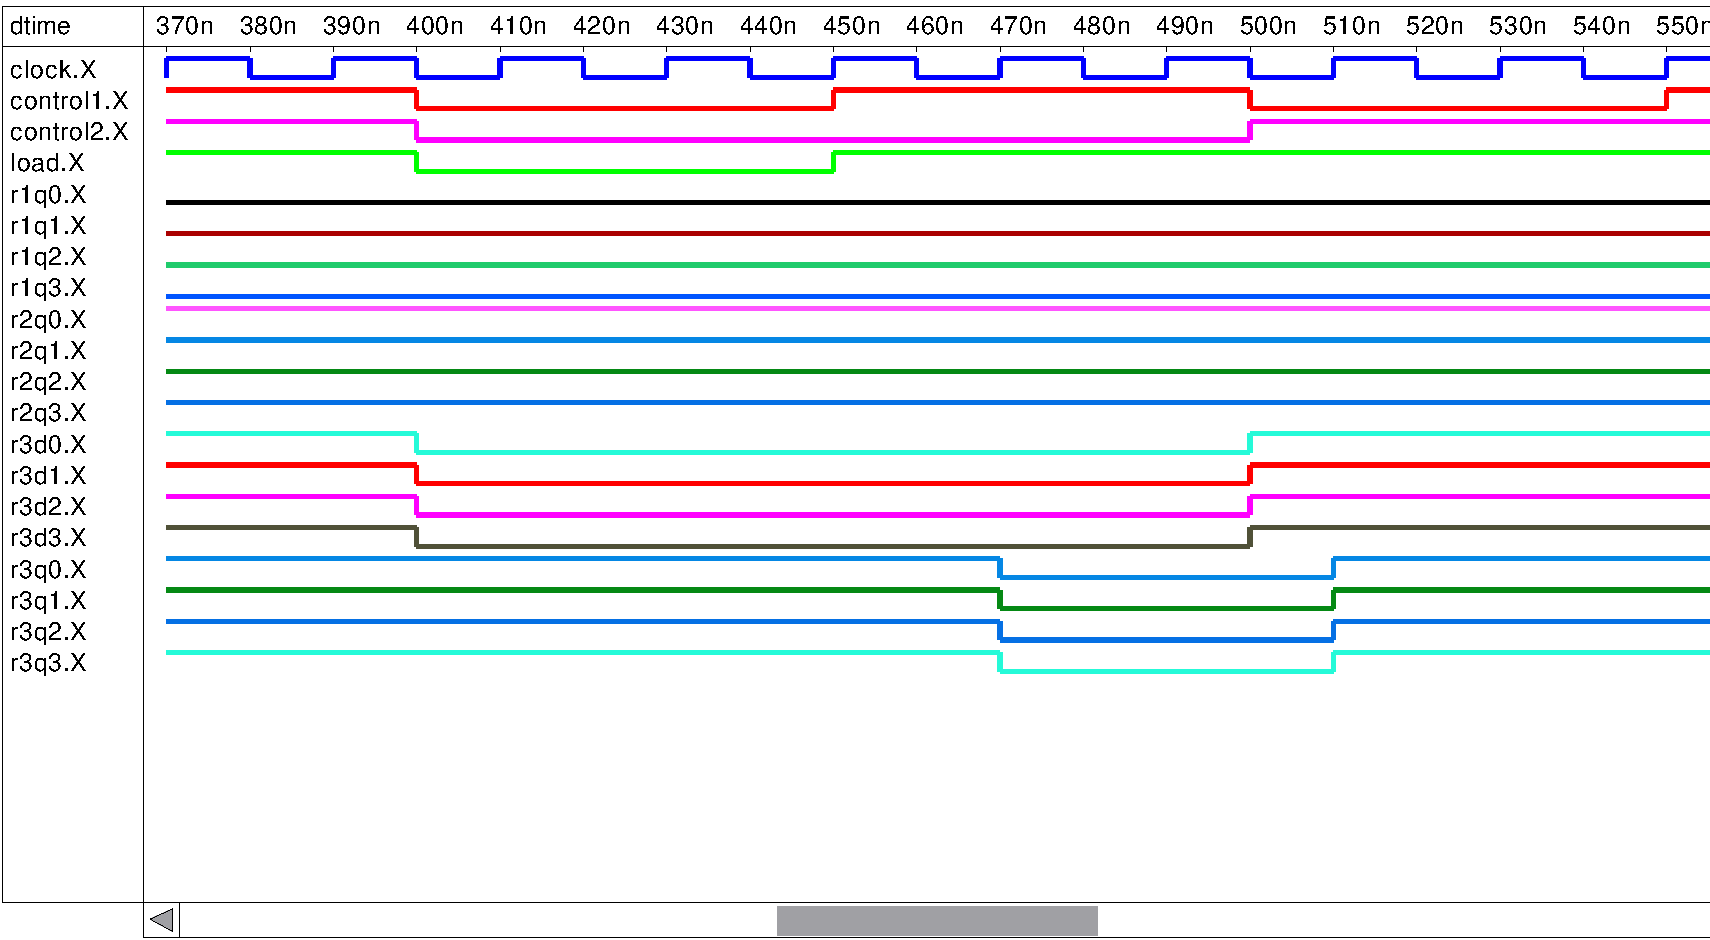
\includegraphics[width=0.9\linewidth]{testrtl}
% quadmuxdpl.png: 99.9998dpi, width=11.40cm, height=6.63cm, bb=0 0 449 261
  \caption{Sample simulation waveforms for RTL design}
  \label{fig:testrtl}
\end{figure} 
\FloatBarrier

\tutsection{End note}

Qucs 0.0.8 adds digital simulation to the impressive list of features
already available in Qucs.  This release represents a significant step
forward in the development of the Qucs project.  The fact that there
are bugs in the first version of the digital simulator is not
surprising given the complexity of the software.  Release 0.0.9 should
go a long way to correcting the most annoying of these bugs.  My
thanks to Michael Margraf and Stefan Jahn for all their encouragement
during the period I tested the Qucs 0.0.8 VHDL generation routines and
the subsequent writing of these notes.
